%%% Fiktivní kapitola s ukázkami citací

\chapter{Návrh}

V~této kapitole si představíme vzhled uživatelských obrazovek, ze kterého vyjdeme při tvorbě uživatelského rozhraní založeného na komponentách knihovny Material UI. Také se budeme věnovat návrhu architektury od extrakce a~uložení dat přes přípravu vyhledávacích indexů až po prezentaci těchto dat v~rámci funkční aplikace.

\section{Návrh uživatelského rozhraní}

Přestože vyvíjíme single-page aplikaci, počítáme s~více obrazovkami pro pohodlnější navigaci. S~využitím knihovny React Router DOM\footnote{https://www.npmjs.com/package/react-router-dom} dokážeme simulovat existenci libovolného množství obrazovek a~zároveň zůstat na jedné stránce bez potřeby opětovného načítání. Tím se odlišíme od tradičních statických aplikací, kterým při každé změně URL včetně query parametrů musí server v~odpovědi poslat odpovídající HTML obsah. Náš přístup má ovšem nevýhodu z~pohledu strojového zpracování, neboť pro vygenerování obsahu stránky potřebujeme v~prohlížeči spustit JavaScript kód. Tím znemožníme zpracování naší aplikace prostřednictvím pouhých HTTP požadavků, což je podstatně jednodušší a~ekonomičtější varianta ve srovnání s~automatizací celého webového prohlížeče. Tento nedostatek ale kompenzujeme transparentním REST API, přes které si lze vyžádat strukturovaná data pomocí HTTP požadavků. Zároveň usnadníme strojové zpracování vyhledávačům, které automatizaci prohlížeče využívají, neboť v~detailech receptů a~ingrediencí zahrneme jejich JSON-LD reprezentaci.

Aplikaci složíme ze $3$ základních uživatelských obrazovek: vyhledávání receptů, detail receptu a~detail ingredience. Všechny obrazovky musí být responzivní a~poradit si s~proměnlivou velikostí obrazovky.

\subsection{Vyhledávání receptů}

Domovskou stránku bude tvořit vyhledávání receptů na základě různých kritérií. Primárně bude k~dispozici výběr požadovaných ingrediencí, sekundárně filtry klíčových slov, kategorií, času přípravy, hodnocení a~nutričních hodnot. Všechny filtry bude možné odstranit samostatně i~najednou pomocí společného tlačítka pro smazání. Pro získání přesnějších výsledků bude při vyplňování filtrů k~dispozici našeptávač, který zobrazí známé možnosti a~spolu s~nimi počty receptů, které jsou při výběru tohoto nastavení k~dispozici. Výsledky budou zobrazovány na stránkách s~$24$ nebo $30$ kartami receptů. Přepínání stránek bude umístěno standardně ve spodní části stránky a~zároveň bude aktuální stránka figurovat v~query parametrech pro přímočarou podporu navigace v~historii prohlížeče. Karta receptu bude obsahovat název, popis, obrázek, hodnocení, počet recenzí, čas přípravy a~počet instrukcí. Navíc bude možné rozbalit seznam ingrediencí, ve kterém budou zvýrazněny aktuálně vyhledávané ingredience. Uživatel bude přesměrován na obrazovku s~detailem receptu při stisknutí tlačítka \texttt{View} nebo při kliknutí na obrázek receptu. Konkrétní rozložení obrazovek viz obrázek \ref{obr02:desktop-search-view} pro desktopová zařízení a \ref{obr02:mobile-search-view} pro mobilní zařízení.

\begin{figure}[p]\centering
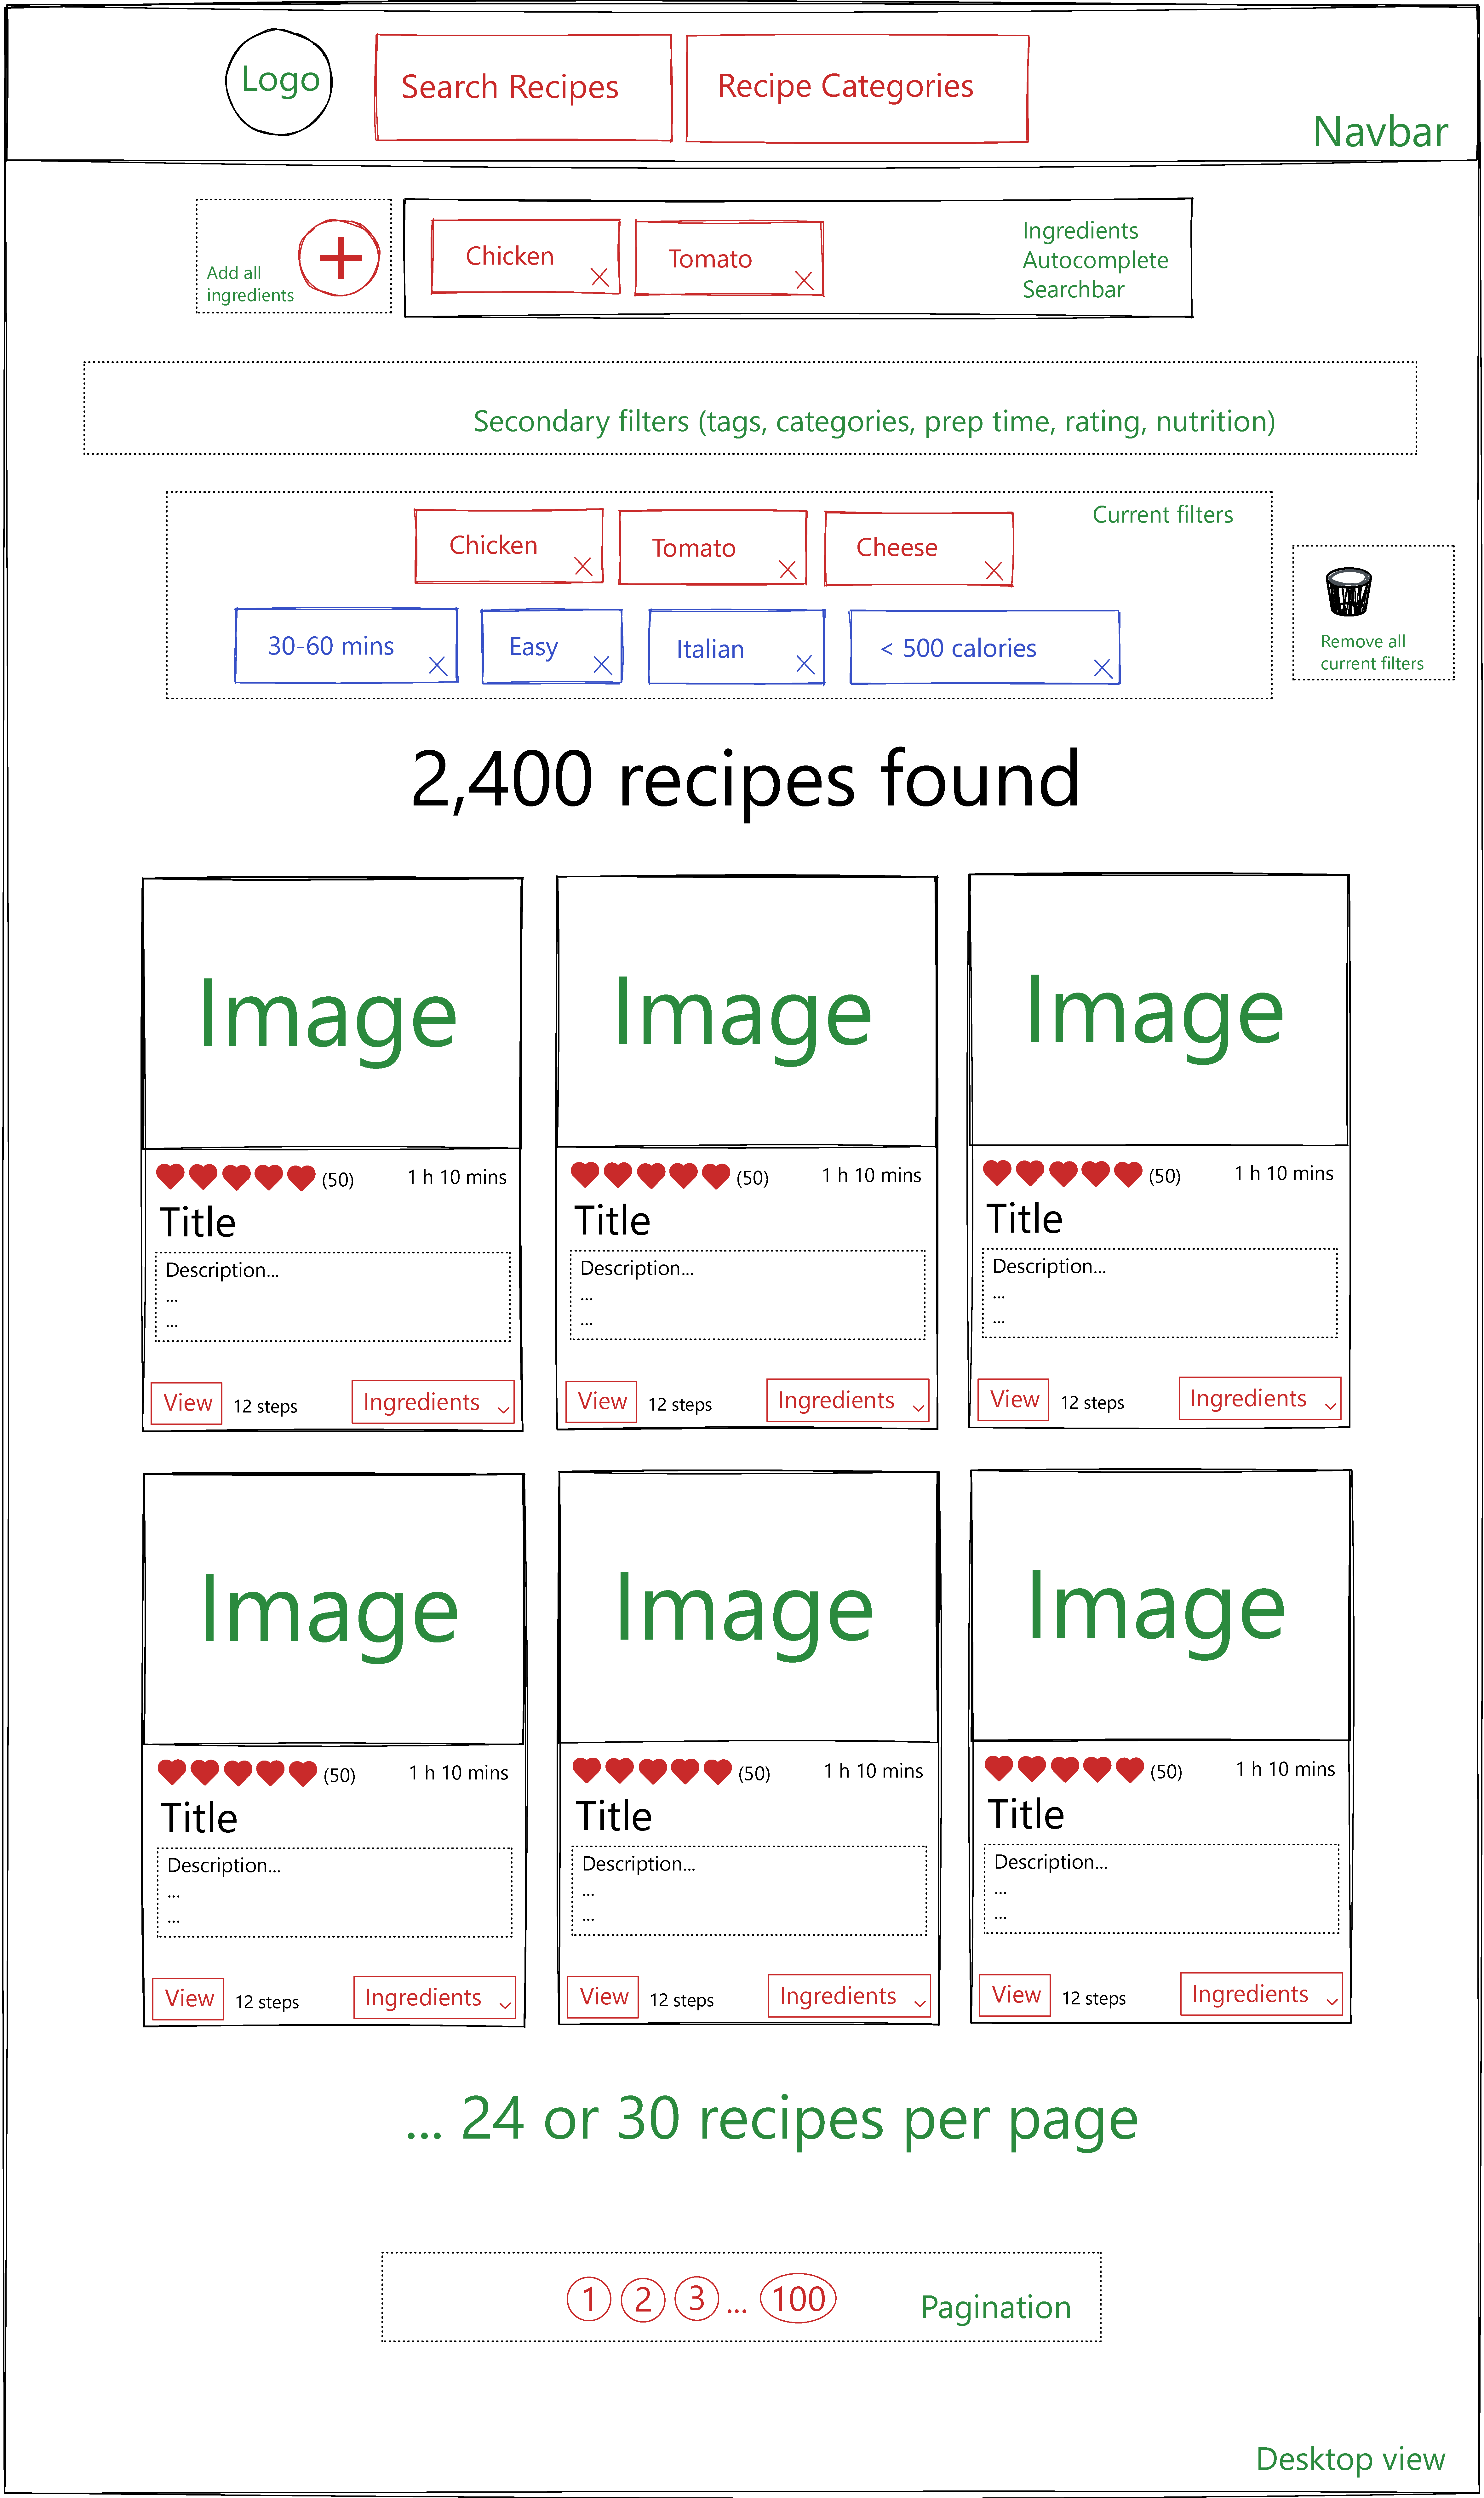
\includegraphics[width=140mm]{../img/desktop-search-view}
\caption{Obrazovka vyhledávání receptů pro desktopová zařízení.}
\label{obr02:desktop-search-view}
\end{figure}

\begin{figure}[p]\centering

\includegraphics[height=230mm]{../img/mobile-search-view}
\caption{Obrazovka vyhledávání receptů pro mobilní zařízení.}
\label{obr02:mobile-search-view}
\end{figure}

\begin{figure}[p]\centering
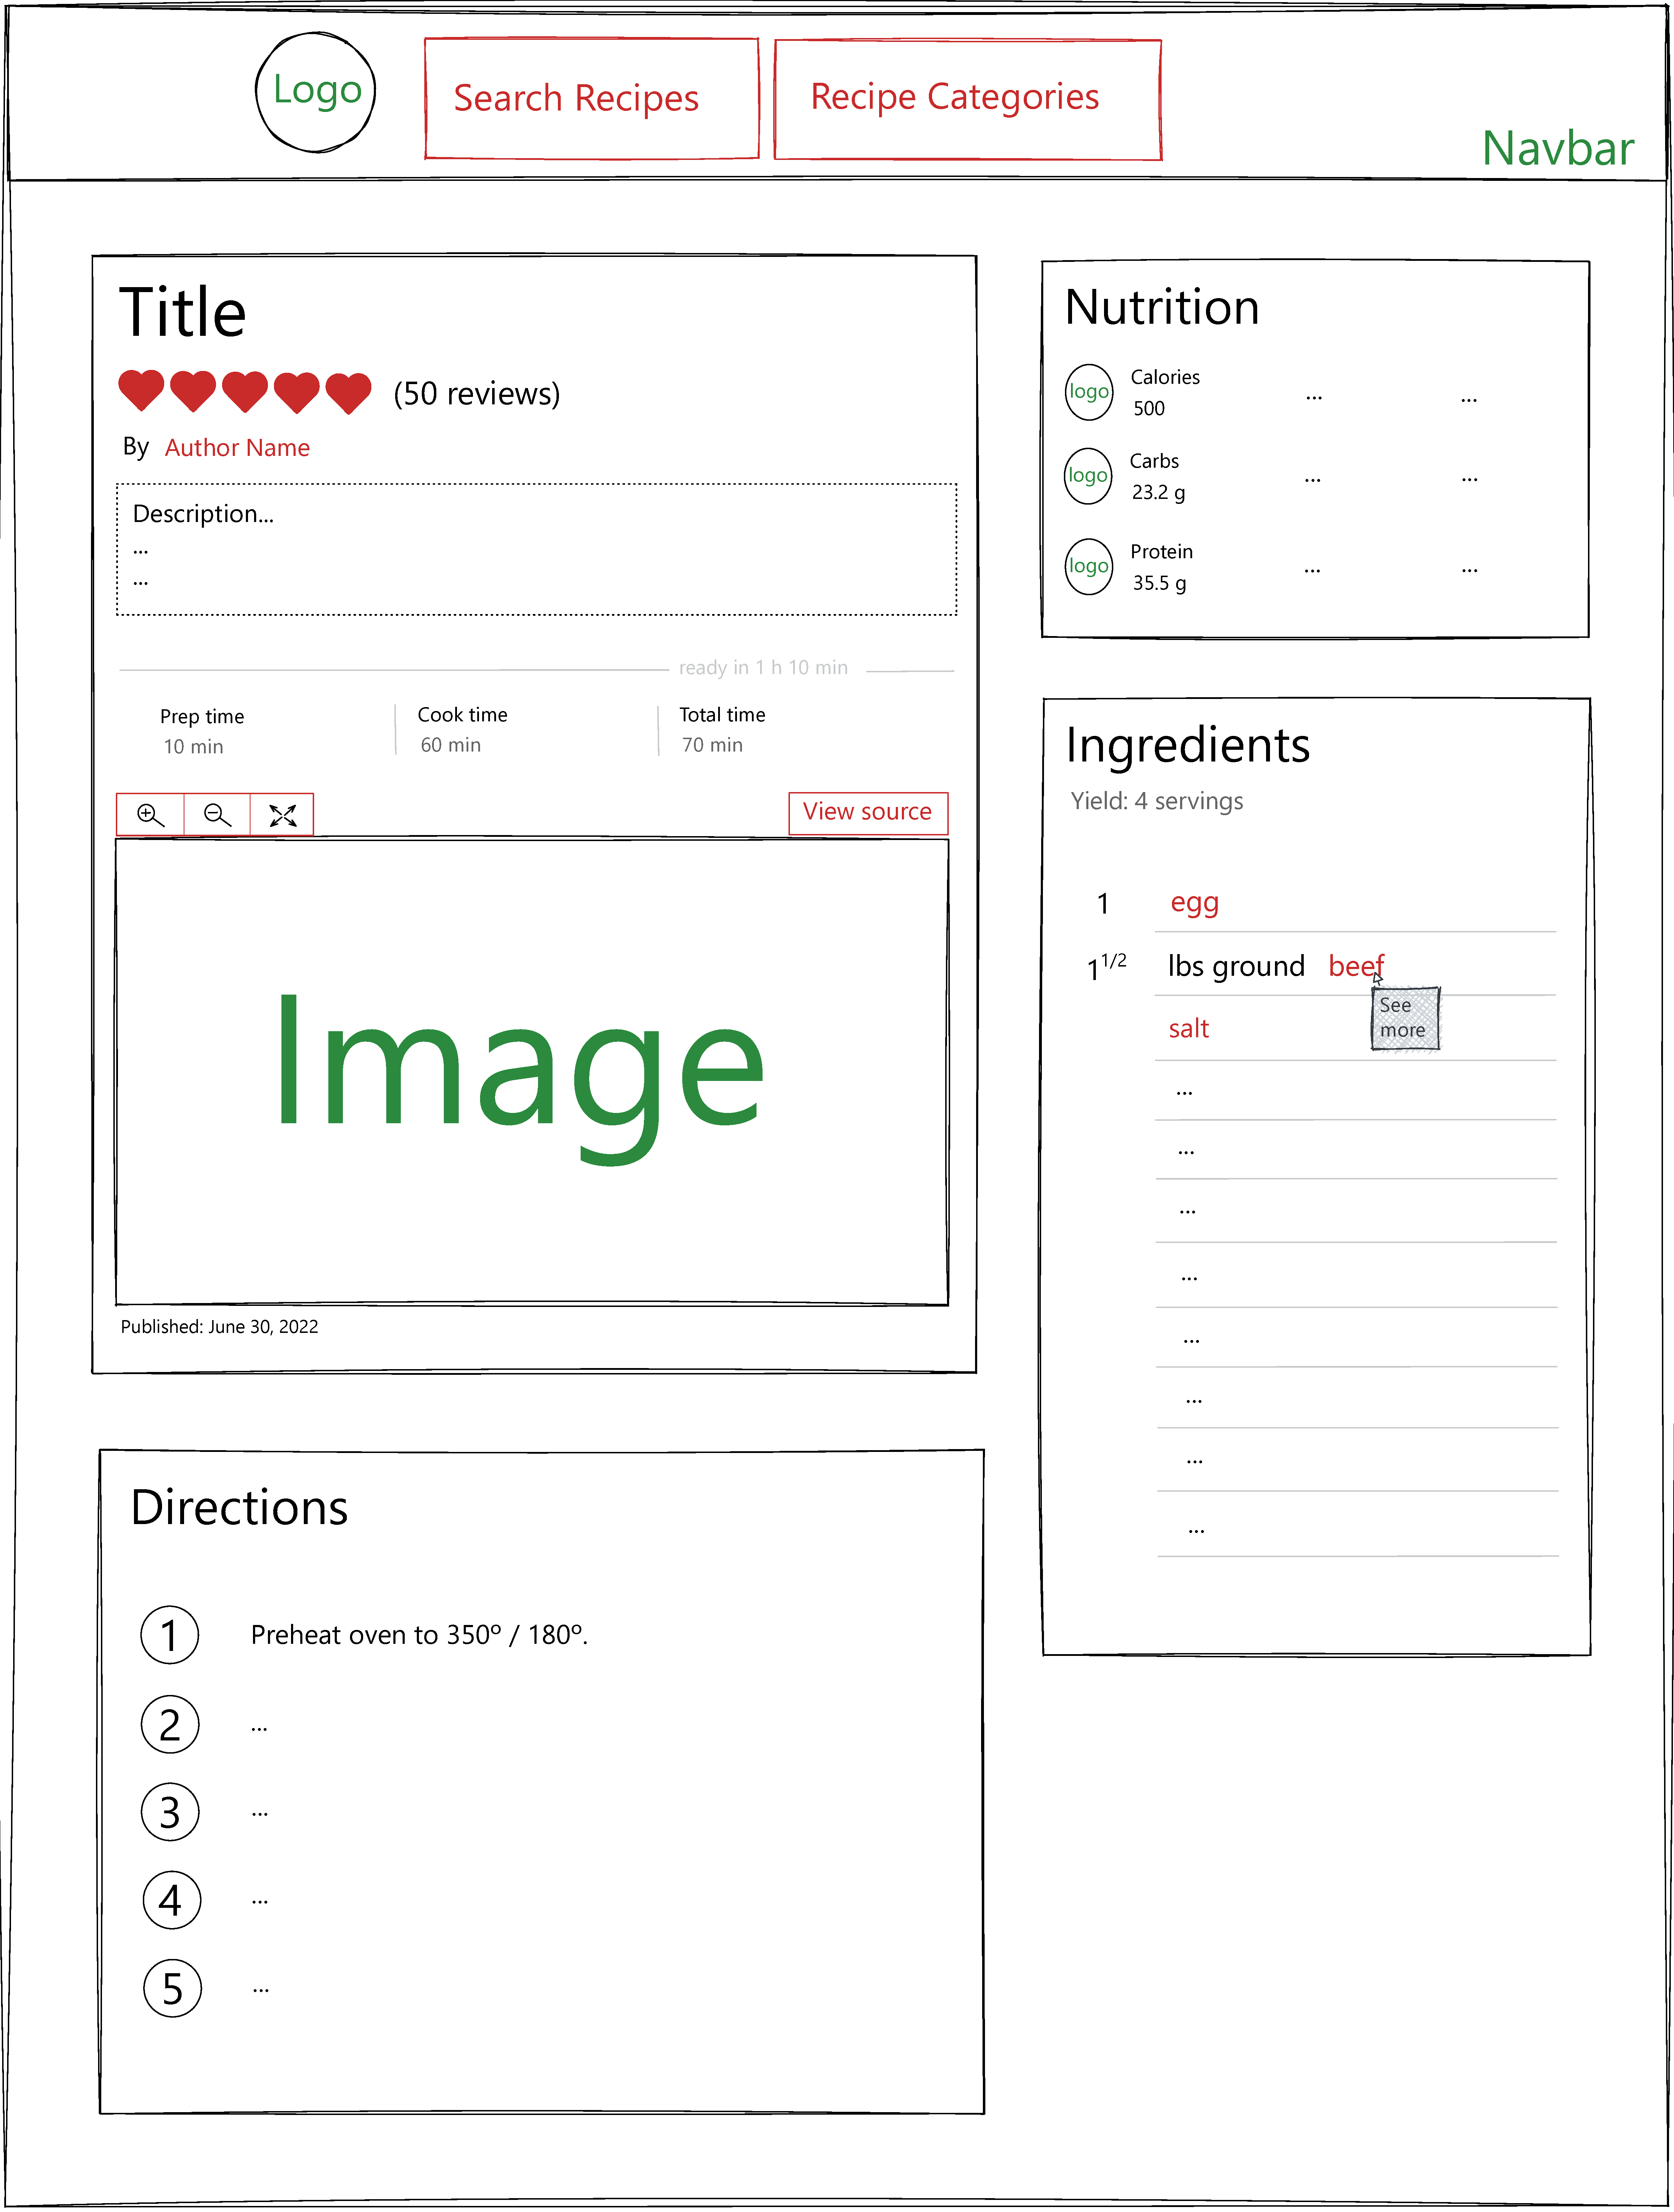
\includegraphics[width=140mm]{../img/detail-view}
\caption{Obrazovka detailu receptu.}
\label{obr02:detail-view}
\end{figure}

\subsection{Detail receptu}

Na obrazovce s~konkrétním receptem bude obsažen název, popis, obrázek, autor, datum publikování, hodnocení s~počtem recenzí, nutriční hodnoty a~samozřejmě ingredience a~postup přípravy. Rozložení pro větší obrazovky viz obrázek \ref{obr02:detail-view}, pro menší obrazovky se všechny karty zobrazí v $1$~sloupci analogicky k~rozložení \ref{obr02:mobile-search-view}. Jako budoucí rozšíření by bylo možné implementovat modul recenzí. V~první fázi by recenze byly pouze extrahovány ze zdrojových datasetů, v~další fázi by uživatelé mohli nové recenze přidávat prostřednictvím naší aplikace.

\subsection{Detail ingredience}

Na obrazovce detailu ingredience budou prezentována data z~otevřených znalostních grafů. Zaměříme se primárně na jméno, popis a~obrázek ingredience, které dle dostupných informací doplníme o~nutriční hodnoty, kategorie, místo původu a~další zajímavosti.

\section{Návrh architektury}

Při návrhu architektury aplikace budeme vycházet z~osvědčené kombinace technologií označované zkráceně jako \emph{MERN}. Pojmenování vzniklo složením prvních písmen klíčových technologií, tedy MongoDB, Express, React a~Node. Pro potřeby naší aplikace se této skupiny nebudeme držet zcela striktně a~systém MongoDB nahradíme rovněž dokumentovým databázovým systémem Apache \,CouchDB. Navíc mezi technologie zařadíme platformu Apache Solr pro pokročilejší vyhledávání receptů. Architektura naší aplikace znázorňující klíčové technologie a jejich propojení je ilustrována schématem \ref{obr02:architecture}. 

\begin{figure}[h!]\centering
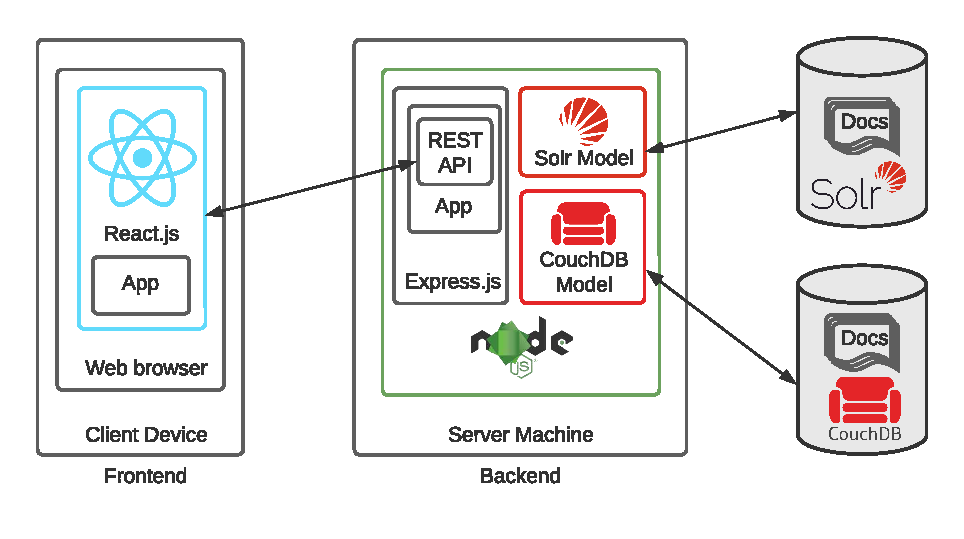
\includegraphics[width=140mm]{../img/architecture}
\caption{Schéma architektury, adaptováno z diagramu MERN aplikace \citep{mern-stack}.}
\label{obr02:architecture}
\end{figure}

Předzpracování dat bude klíčovou fází řešení spolu s~prezentační vrstvou na straně klienta. Serverová část aplikace bude vystupovat pouze jako prostředník mezi klientem a~databází, respektive platformou Solr pro vyhledávací dotazy. Jejím úkolem bude zprostředkování požadovaných dat z~perzistovaného úložiště, která téměř beze změny předá klientovi. Tento přístup si vybere daň v~podobě obsáhlejší databáze, neboť budeme ukládat i~taková data, která bychom dokázali vygenerovat z~ostatních informací. Nejdůležitější instancí tohoto opakování dat bude uložení JSON-LD reprezentace a~zároveň strukturovaných dat v~rámci každého dokumentu receptu. Strukturovaná data by bylo možné při každém dotazu odvodit z JSON-LD nebo naopak. Přesunuli bychom ale komplexitu převodu z~jednorázové fáze předzpracování na samotnou aplikaci, ať už na straně serveru či klienta. Příprava dat pro prezentaci by navíc při každém dotazu trvala o~něco déle, což by se při větším množství dat mohlo negativně odrazit na svižnosti aplikace a~tranzitivně na uživatelském zážitku.

\subsection{Příprava dat}

V~předchozí kapitole jsme si představili řadu alternativ pro získání datasetů s~recepty a~následně doplňujících informací k~ingrediencím. Dle požadavků aplikace potřebujeme minimálně $50\,000$ receptů z~aspoň $2$ různých zdrojů. Také vyžadujeme integraci $2$ nebo více znalostních grafů s~otevřenými daty. Nemáme spodní limit na počet ingrediencí, které musíme ze znalostních grafů extrahovat. Záleží totiž na úspěšnosti propojení našich ingrediencí s~entitami ze znalostních grafů, která se projeví až při praktickém testu.

Přípravu dat můžeme dále rozdělit na $2$ základní fáze a~to extrakci a čištění dat. Ne všechna data jsou totiž vhodná pro přímou prezentaci uživateli. Jak jsme zmiňovali v~minulé kapitole, volně dostupné datasety s~recepty často cílí spíše na oblast strojového učení. Extrahovaná data je tedy potřeba manuálně zkontrolovat a navrhnout heuristiku, pomocí které bude většina dat normalizována, případně odstraněna při nesplnění zadaných kritérií. Vzhledem k charakteru problému a~omezené časové dotaci nelze na každou datovou sadu aplikovat deterministické řešení, které by eliminovalo všechny anomálie, proto se v~některých případech musíme spokojit s~heuristikou.

\subsubsection{Extrakce dat}

Na tomto místě je vhodné rozhodnout, které ze zdrojů dat popsaných v~předchozí kapitole nakonec použijeme v~rámci našeho řešení. U~dat k~ingrediencím máme na výběr znalostní grafy DBpedia a~Wikidata, případně méně obsáhlý RDF dataset z~projektu FoodKG. Pro maximalizaci počtu nalezených výsledků se zaměříme na grafy DBpedia a~Wikidata. V~kategorii receptů zvolíme kombinaci statických datových sad s~recepty a~generování vlastních datasetů pomocí procesu web scraping. Během implementace vlastní extrakce dat zapojíme knihovnu Apify pro Node.js a~její koncept tzv.~\emph{actorů}, což jsou programy určené primárně pro cloudovou platformu Apify, kde jsou spouštěny uvnitř Docker kontejnerů. Mohou mít za úkol automatizaci libovolných úkonů prováděných ve webovém prohlížeči, od jednoduchého posílání e-mailů až po extrakci dat z~komplexních webových stránek. Actory lze pomocí nástroje Apify CLI\footnote{https://www.npmjs.com/package/apify-cli} spouštět i~lokálně, čehož pro jednodušší konfiguraci využijeme v~našem řešení.

\paragraph{Food.com}\mbox{}\\

Vzhledem k~požadavkům definovaným v~předchozí kapitole nám bude vyhovovat dataset Food.com Recipes and~Interactions dostupný na platformě Kaggle, z~něhož jsme schopni získat přibližně $180\,000$ identifikátorů receptů a~také seznam normalizovaných ingrediencí. Dle provedené analýzy není vhodné použít textová data v~prezentační vrstvě vzhledem k jejich lowercase formátu. Navrhneme tedy řešení z~oblasti web scrapingu, které na vstupu přijme URL adresy s~detaily receptů, na každou adresu odešle požadavek GET a~z~HTML odpovědi extrahuje JSON-LD data. Program bude mít možnost získat přes CSS selektory libovolná data z~načteného HTML, pokud by v JSON-LD reprezentaci nebyla obsažena, nebo byla méně strukturována. Programu tedy přidělíme také zodpovědnost za tvorbu strukturovaných dat, která do vygenerovaného datasetu uloží ke každému receptu spolu s~jeho JSON-LD podobou. Strukturovanými daty zde rozumíme čas přípravy, počet porcí, klíčová slova, která jsou v~JSON-LD uložena ve společném řetězci namísto pole řetězců, hodnocení receptu s~počtem recenzí, nutriční hodnoty s~jednotkami měření a~ingredience s~množstvím a~jednotkou oddělenými od ostatního textu.

Extrahované výsledky uložíme do společného JSON souboru, který následně sloučíme s~informacemi z~datasetu Food.com Recipes and~Interactions. Poskytnutý JSON-LD například neobsahuje kompletní informace o~autorovi, ale pouze jeho jméno. Dle samotného jména nejsme schopni autora jednoznačně identifikovat a~zjistit odkaz na jeho profil v~rámci aplikace Food.com. URL adresa autora je totiž sestavena z~jeho unikátního id, které máme k~dispozici právě v~datasetu z~Kaggle. Dále budeme chtít extrahované recepty rozšířit o~normalizované ingredience, abychom nemuseli navrhovat vlastní heuristiku a~usnadnili si pozdější mapování ingrediencí na entity ze znalostních grafů. Po sloučení všech potřebných dat provedeme finální čištění a následně recepty jako JSON dokumenty uložíme do databáze.

Výše popsané řešení extrakce dat z~Food.com má nevýhodu z~pohledu škálovatelnosti. Maximální počet receptů, které jsme schopni získat, je roven počtu receptů v~datasetu z~Kaggle. Celkový počet receptů na stránce Food.com se od doby pořízení datasetu zvětšil více než dvakrát na aktuálních $526\,851$ receptů. Nicméně i~s~naším zjednodušeným programem vyžadujícím připravené URL adresy detailů receptů jsme schopni získat téměř kompletní data. Zmíněný dataset Recipe1M+ v~době psaní této práce obsahuje téměř $510\,000$ URL adres receptů z~aplikace Food.com. Při potřebě většího škálování bychom mohli využít tato URL, neměli bychom k~nim ovšem normalizované ingredience a~byli bychom omezeni striktně akademickým využitím. Pro účely naší práce se spokojíme s~horní hranicí $180\,000$ receptů s~normalizovanými ingrediencemi. Tyto recepty jsou dle autorů datasetu Majumdera a~kol. podmnožinou receptů z~let $2000$-$2018$, které mají aspoň $3$~kroky postupu a~počet ingrediencí v rozmezí $4$ a $20$ \citep{majumder-etal-2019-generating}. Kód souvisejícího projektu pro generování personalizovaných receptů je dostupný jako open-source na platformě GitHub, lze tedy předpokládat, že datovou sadu lze využívat bez omezení.

\paragraph{Allrecipes}\mbox{}\\

Jako další zdroj receptů si vybereme webovou aplikaci Allrecipes. Pro ni sice nemáme k~dispozici podrobný dataset jako u~stránky Food.com, vystačíme si ale s~vlastní extrakcí dat prostřednictvím Apify actora. Mohli bychom využít prakticky stejnou šablonu, jako u~programu pro zpracování Food.com. S~využitím datasetu Recipe1M+ dokážeme získat $49\,000$ URL adres detailů receptů. Poměrně snadno bychom ale dokázali navrhnout pokročilejší řešení extrakce dat, které by dynamicky procházelo celou webovou stránku Allrecipes, našlo detaily všech receptů a~z~nich extrahovalo aktuální data. Tímto přístupem bychom odstranili závislost na datové sadě Recipe1M+ a~získali větší počet výsledků, ale pro nalezení všech receptů bychom museli zpracovat více požadavků. Celkový počet receptů na Allrecipes se aktuálně pohybuje kolem $50\,000$, což lze zjistit spuštěním vyhledávání bez jakýchkoli nastavených filtrů. Jednou z možností by bylo projít všechny kategorie, jinou zase využití interního API z vyhledávací stránky, přes které lze získat URL adresy $24$ receptů v~rámci $1$~požadavku.

Webová aplikace Allrecipes nabízí svým uživatelům ve vztahu k~ingrediencím vyhledávání dle surovin a~také možnost přizpůsobit množství ingrediencí požadovanému počtu porcí. Tato skutečnost naznačuje, že si aplikace přísady interně spravuje ve strukturované podobě, přestože v~přiloženém JSON-LD je poskytuje jako prostý text včetně množství a jednotky měření. Zaměřme se na konkrétní ingredienci uvnitř HTML dokumentu vybraného receptu. Můžeme si povšimnout, že v~atributech příslušného \texttt{input} elementu jsou uložena strukturovaná data ingredience v~následujícím formátu (ukázka z~receptu \texttt{92462} pro surovinu kuřecí vývar):

\begin{code}
<input
    class="checkbox-list-input"
    data-tracking-label="ingredient clicked"
    data-quantity="½"
    data-init-quantity="0.5"
    data-unit="cup"
    data-ingredient="chicken broth"
    data-unit_family="volumetric"
    data-store_location="Soup"
    type="checkbox"
    value="(14.5 ounce) can chicken broth"
    id="recipe-ingredients-label-92462-0-4">
\end{code}
%$

Z atributů elementu \texttt{input} dokážeme rozpoznat název, množství i~jednotku ingredience. Díky tomu získáme ještě přesnější data, než prostřednictvím normalizovaných ingrediencí z~datasetu Food.com Recipes and~Interactions.

\paragraph{Znalostní grafy}\mbox{}\\

V~první fázi extrakce dat ze znalostních grafů, ať už DBpedia či Wikidata, potřebujeme identifikovat entity ingrediencí, které dokážeme namapovat na jména surovin z~jednotlivých receptů. Pro každou entitu ingredience vyjádřenou pomocí IRI pak extrahujeme vybrané informace. U grafu DBpedia budeme cílit především na:
\begin{itemize}
    \item jméno
    \item popis
    \item obrázek
    \item kategorie
    \item místo původu
\end{itemize}

Z~nutričních hodnot se zaměříme na energii v~kaloriích nebo kilojoulech, dále na obsah tuku, sacharidů, bílkovin, vlákniny, cholesterolu a~cukru. Aktuálně se zabýváme pouze anglickou lokalizací aplikace, všechna textová data tedy omezíme na anglické výsledky. Jedinou povinnou informací bude název (label) ingredience, všechna ostatní data budou nepovinná, neboť se formát i~množství dat napříč ingrediencemi výrazně liší.

\subsubsection{Čištění dat}

V~rámci fáze čištění dat potřebujeme extrahovaná data převést do formátu vhodného k~prezentaci koncovému uživateli. Jednotlivé kroky procesu čištění mohou být rozloženy do více míst přípravy dat. Již během extrakce dat probíhá odstranění mezer a~znaků nového řádku na okrajích řetězců. Dále je potřeba se vypořádat se znaky, které jsou kvůli vnoření v~HTML dokumentu kódovány jinými znaky, aby bylo zajištěno jejich korektní zobrazení. Takové znaky se vyskytují např. v~extrahovaných JSON-LD dokumentech, před jejich uložením do databáze tedy provedeme dekódování. Rekurzivně projdeme obsah každého objektu načteného z~JSON-LD dokumentu a~všechny řetězce dekódujeme s~využitím open-source knihoven pro Node.js. V~našem řešení integrujeme knihovny \texttt{html-escaper} a~\texttt{html-entities} dostupné přes správce balíčků npm.

Dále jsme se rozhodli z~vyhledávání vyřadit recepty bez fotografie, které lze identifikovat a~přeskočit již během fáze extrakce nebo následně při ukládání do databáze, případně až při tvorbě dokumentů pro vyhledávací platformu Solr. Zvolíme poslední způsob, recepty tedy uložíme do vlastní databáze bez ohledu na přítomnost jejich obrázků. Díky tomu budeme mít v~budoucnu snadnou cestu k~využití zbývajících receptů bez fotografií, ať už pro účely strojového učení nebo i~zobrazení uživateli, pokud by větší nabídka receptů výrazně převážila nevýhodu absence ilustračních fotografií.

Také data k~ingrediencím budou vyžadovat významné čištění. V~datasetu Food.com Recipes and~Interactions máme k~dispozici přibližně $8\,000$ unikátních ingrediencí. Co nejvíce z~nich bychom chtěli nabídnout uživateli v~rámci našeptávače ve vyhledávání dle ingrediencí. Pro tento účel názvy ingrediencí převedeme do estetičtějšího formátu s~velkým počátečním písmenem. Po manuální kontrole seznamu ingrediencí ale narazíme na řadu slov, která se mezi suroviny dostala omylem vlivem chybného parsování jmen ingrediencí. Nebudeme zde uvádět kompletní výčet, typicky se ale jedná o~názvy jednotek měření nebo obecné fragmenty ingrediencí, které samy o~sobě žádnou ingredienci nepředstavují (např. samostatná slova \texttt{clove}, \texttt{seed}, \texttt{extract}, která by byla validní pouze v~kontextu typu \texttt{garlic clove}, \texttt{sesame seed} a~\texttt{vanilla extract}). Vzhledem k~velkému počtu ingrediencí navrhneme heuristiku čištění pomocí regulárních výrazů. Zaměříme se zejména na nejčastěji používané ingredience, které budou zobrazeny v~horní části našeptávače. Pro potřeby našeptávače nastavíme limit maximálního počtu slov ingredience a~to na hodnotu $3$. Pro mapování na entity ze znalostních grafů ale využijeme původní sadu ingrediencí bez omezení počtu slov.

S~normalizovanými ingrediencemi z~Food.com Recipes and~Interactions souvisí další problém --- nejsou přiřazeny ke všem receptům z~datasetu. Texty surovin sice využijeme z~extrahovaného JSON-LD, normalizované ingredience ale potřebujeme k~propojení s~informacemi z~grafů DBpedia a~Wikidata. Recepty bez normalizovaných ingrediencí tedy musíme projít a~pro každou jejich přísadu zkusit na základě prostého textu nalézt co nejbližší shodu s~některou z~normalizovaných ingrediencí. Pro zjednodušení budeme akceptovat pouze přesné shody, přestože nám tímto způsobem může část ingrediencí uniknout, neboť mohou být v~prostém textu uvedeny v~jiném pádě nebo čísle.

Dalším úkolem čisticí fáze bude normalizace JSON-LD reprezentace ingrediencí z~grafu DBpedia. Ve srovnání s~projektem Wikidata jsme zde ve výhodě, jelikož data obdržíme přímo v JSON-LD. Zároveň ale extrahujeme data pro více ingrediencí najednou a~každá z~nich má vlastní schéma, které se většinou plně neshoduje s~ostatními entitami. Při skupinové extrakci dat se ale musí vytvořit univerzální schéma, kterým lze vyjádřit všechny obsažené informace. Naším úkolem bude projít uložené kolekce ingrediencí a~pro každou ingredienci vytvořit minimální JSON-LD kontext, kterým ji lze popsat. Jednotlivé ingredience pak do databáze uložíme vždy s~vlastním JSON-LD kontextem. V~praxi se totiž často stává, že objevíme pod stejnou vlastností různé typy hodnot. Např. region původu ingredience může nést IRI příslušné entity z~grafu DBpedia, ale také prostý literál. Skutečný typ musí být řádně definován kontextem JSON-LD dokumentu. Proto není vhodné mít společný kontext pro všechny ingredience, neboť by u~některých vlastností existoval duplicitní popis použitých typů.

\subsection{Databázový model}

Pro uložení dat receptů a~ingrediencí zvolíme dokumentovou databázi Apache CouchDB, často označovanou zkráceně CouchDB. Nejbližší alternativou z~řad NoSQL dokumentových databází by byl systém MongoDB, který je stejně jako databáze CouchDB open-source. Pro naše potřeby by dobře fungoval libovolný z~těchto systémů, neboť chceme využít zejména konceptu dokumentových databází, které typicky nevyžadují striktní schéma a~umožňují tak kompaktní uložení různorodých dat ve formátu JSON. To je v~naší doméně cenná vlastnost, neboť plánujeme ukládat data poměrně komplexní struktury --- vezměme v~potaz například JSON-LD formát s~mnoha zanořenými objekty. Také extrahujeme data z~více zdrojů a~vyžadování zcela jednotného rozhraní by nám v~některých situacích zbytečně zkomplikovalo práci. Na základě jakého kritéria tedy rozhodujeme mezi variantami CouchDB a~MongoDB?

Databázi budeme pokládat pouze velmi jednoduché dotazy, totiž vyžádání dokumentu na základě jeho unikátního id. Pro práci s~databází preferujeme použití Node.js knihovny, což je splnitelné oběma databázovými systémy CouchDB i~MongoDB, neboť oba poskytují oficiální ovladač pro Node.js. K~obsluze složitějších vyhledávacích dotazů využijeme systém Apache Solr, který si bude držet vlastní podmnožinu dat z~dokumentů uložených v~databázi. Kombinací Apache CouchDB s~Apache Solr bychom sjednotili technologie z~dílny Apache Software Foundation. Zároveň by se nám v~budoucnu mohla hodit podpora současného čtení a~zápisu, kterou systém CouchDB nabízí \citep{mongodb-vs-couchdb}. Co se týče dat s~recepty či ingrediencemi, není potřeba vyžadovat, aby se uživateli vždy zobrazila verze se všemi aktualizacemi. Např. vybraný recept zůstává relevantní i~v~momentě, kdy zrovna současný nebo jiný uživatel přidává k~receptu nové hodnocení. Díky systému verzování dokumentů, který CouchDB implementuje, se nemusíme obávat o~dostupnost dat během jejich aktualizace.

V~systému CouchDB lze snadno vytvářet a~spravovat více databází neboli kolekcí dokumentů. Vytvoříme tedy samostatné databáze pro recepty a~ingredience, přičemž oba typy dokumentů v~sobě budou mít uložena strukturovaná data i~JSON-LD reprezentaci. Na rozdíl od tradičních relačních databází nemusíme předem definovat žádná schémata ukládaných dat.

S~CouchDB můžeme komunikovat přes webové rozhraní skrze přehlednou aplikaci Fauxton, pomocí REST~API nebo prostřednictvím již zmíněné knihovny v~prostředí Node.js. Pro automatizované nahrávání dokumentů využijeme oficiální knihovnu \texttt{nano}. S~velikostí našeho projektu si můžeme dovolit při nahrávání nových dat nejprve stávající data odstranit a~poté je vložit do čisté databáze. Kdybychom totiž chtěli dokumenty aktualizovat, potřebovali bychom u~každého z~nich poskytnout aktuální verzi, což by pro přepsání celé databáze byl zbytečně komplikovaný postup. S~rostoucím počtem dokumentů bychom ale nejspíše museli přistoupit na aktualizaci dat namísto jejich odstraňování a~opětovného nahrávání, neboť již pro přidání kolekce o~velikosti $50\,000$ dokumentů se pohybujeme v~řádu delších minut.

\subsection{Indexy}

Pro uložení dokumentů do databáze CouchDB není potřeba specifikovat žádné schéma. Během konfigurace platformy Apache Solr pro vyhledávání se ovšem bez striktně definovaného schématu neobejdeme. Respektive abychom byli přesní, Solr dokáže na základě vložených dat odvodit schéma dynamicky, často ale nezvolí datový typ správně a~navíc je při výběru zbytečně generický. Představme si libovolný řetězec z~dokumentu receptu, například text jedné ingredience. Pokud Solr nenajde ve schématu žádnou definici typu u~vlastnosti ingredience, vytvoří pro ni dynamický index typu \texttt{string}. Na první pohled se zdá být vše v~pořádku, když si ale projdeme dostupné typy, najdeme mezi nimi i~podstatně specifičtější variantu \texttt{text\underline{{ }}en}. Typ anglického textu je pro naši aktuální lokalizaci ideální, neboť nabízí vestavěnou podporu skloňování a~časování anglických slov. V~praxi nám pomůže najít více relevantních výsledků. Uživatel může zadat například ingredienci \texttt{tomatoes}, Solr provede normalizaci vyhledávaného termínu a~vrátí recepty obsahující mezi surovinami nejen slova \texttt{tomatoes}, ale také \texttt{tomato}.

Prvním krokem pro práci s~platformou Solr je tedy kompletní návrh schématu pro dokumenty receptů. Pro vytvoření schématu využijeme skript operující nad REST~API poskytovaným systémem Solr, čímž proces automatizujeme a~usnadníme případnou migraci na jiné zařízení. Solr umožňuje data rozdělit do tzv.~jader, založíme tedy samostatné jádro pro dokumenty s~recepty a~vytvoříme infrastrukturu, která umožní snadné přidání nového jádra, pokud by v~budoucnu bylo potřeba. V~rámci současných požadavků aplikace by se mohlo zdát, že budeme vyhledávací schopnosti platformy Solr potřebovat i~pro dokumenty ingrediencí, konkrétně pro řešení našeptávače surovin. Seznam doporučených přísad by se totiž měl aktualizovat na základě vstupu uživatele. Po napsání každého nového znaku se musí zobrazit pouze ingredience, které odpovídají vyhledávanému výrazu. Přirozeně nebereme v~potaz velikost písmen a~vzhledem k~výhradně anglické lokalizaci se v~současnosti nezabýváme ani diakritikou. Využití systému Solr by nám pomohlo nabídnout více relevantních ingrediencí, neboť bychom vyhledávaný výraz mohli interpretovat jako anglický text a~poradit si tak s~jeho formátem v~různých tvarech a časech. Kvůli každému napsanému znaku bychom ale museli odeslat dotaz serveru hostícímu instanci Solr, což by generovalo poměrně významné zpoždění vlivem komunikace po síti. Spokojíme se tedy s~jednodušší architekturou našeptávače --- vyžádáme si všechny ingredience najednou a~zobrazení relevantních návrhů během psaní vyřešíme na straně klienta. Jak lze ale získat seznam všech unikátních ingrediencí, pokud máme v~Solr uloženy pouze dokumenty receptů? Odpovědí je fasetové vyhledávání.

\subsubsection{Fasetové vyhledávání}

Fasetové vyhledávání, označované také jako fasetová navigace, je způsob interakce, během které uživatel filtruje výsledky výběrem validních hodnot fasetového klasifikačního systému. Tento styl vyhledávání nevyžaduje hierarchické uspořádání nabízených možností, díky čemuž lze filtry přidávat i~odebírat v~libovolném pořadí. Navíc uživatel typicky předem zná počet výsledků, které se po aplikování daného filtru zobrazí \citep{faceted-search}. V~kontextu naší aplikace se fasetová navigace hodí pro jednotlivé vlastnosti vyhledávání, jakými jsou nejen ingredience, ale také klíčová slova, kategorie, typ kuchyně, čas přípravy či hodnocení. Každý z~těchto filtrů je zcela nezávislý, není tedy žádoucí vytvářet kolem nich hierarchii. Nedávalo by smysl zpřístupnit například vyhledávání dle ingrediencí až po výběru kategorie receptu. Na druhou stranu, výběr kategorií může ovlivnit (respektive omezit) nabídku ingrediencí ve fasetové navigaci a~stejně tak volba určitých ingrediencí může vyřadit některé kategorie receptů.

Platforma Solr poskytuje přímou podporu fasetové navigace nad libovolnými položkami dokumentů. Můžeme tedy například snadno specifikovat fasetové vyhledávání nad ingrediencemi, čímž získáme list unikátních jmen surovin, které se v~celé kolekci receptů vyskytují. Je zde ovšem jisté omezení. Pokud fasetové vyhledávání spustíme přímo nad ingrediencemi, které máme uloženy pod typem anglického textu, Solr nám vrátí pouze transformovaná jména ingrediencí, tak jak je má uložena pro své interní vyhledávání. Data tohoto formátu nejsou vhodná pro prezentaci uživateli, tudíž budeme potřebovat ke každému receptu přiřadit nový seznam ingrediencí určený výhradně pro fasetové vyhledávání. Na úrovni schématu definujeme typ fasetových ingrediencí jako prostý řetězec, nad kterým se neprovedou žádné transformace.

\subsubsection{Zvýraznění nalezených výrazů}

Dalším konceptem, se kterým se během vyhledávání pomocí Solr setkáme, bude tzv. \emph{highlighting} neboli zvýraznění vyhledaných výrazů. Využijeme jej při prezentaci surovin jakožto primárního filtru. U~libovolného receptu na vyhledávací obrazovce bude možné zobrazit kompletní seznam ingrediencí. Pro lepší přehlednost zvýrazníme aktuálně vyhledávané ingredience tučným písmem a~pro přesnou identifikaci těchto pojmů využijeme vestavěnou funkci od platformy Solr. Informace o~zvýrazněných ingrediencích doručíme na frontend aplikace spolu s~dokumenty receptů.

\subsubsection{Model receptu}

Schéma receptu navrhneme dle požadavků na vlastnosti, podle kterých potřebujeme recepty vyhledávat. Zároveň zde ale patří definice všech položek, které budeme na vyhledávací stránce zobrazovat. Teoreticky bychom mohli platformu Solr využít pouze na vyhledání identifikátorů receptů na základě zadaných indexů a~ostatní informace získat z~databáze CouchDB. Tento přístup by optimalizoval množství paměti využívané systémem Solr a~odstranil poměrně výraznou duplicitu dat. Na druhou stranu by do zpracování vyhledávacích dotazů zanesl větší komplexitu a~časovou prodlevu, která by vznikla nadbytečnou komunikací s~\,CouchDB. Pokud si budeme všechny potřebné informace pro vyhledávací stránku držet v~systému Solr, bude nám stačit zpracovat pouze jeden vyhledávací dotaz pro zobrazení jedné stránky receptů. Rychlé vyhledávání je klíčovou funkcionalitou naší aplikace, proto zde upřednostníme optimalizaci časové složitosti namísto paměťové.

Schéma dokumentu receptu uloženého v~Solr bude následující (jedná se pouze o~ilustrační schéma, kde typy odpovídají standardním typům dle specifikace Solr, nikoli běžně dostupným typům formátu JSON):

\begin{code}
{
    name: text_en,
    description: text_en,
    recipeCategory: text_en,
    ingredients: text_en,
    tags: text_en,
    rating: pfloat,
    reviewsCount: pint,
    stepsCount: pint,
    cookMinutes: pint,
    prepMinutes: pint,
    totalMinutes: pint,
    image: string,
    date: string,
    calories: pint,
    fat: pfloat,
    saturatedFat: pfloat,
    cholesterol: pfloat,
    sodium: pfloat,
    carbohydrate: pfloat,
    fiber: pfloat,
    sugar: pfloat,
    protein: pfloat,
}
\end{code}
%$

Ne všechny obsažené položky nutně využijeme v~první verzi naší prezentační vrstvy (například datum a~počet minut samotné přípravy či vaření pokrmu). Jejich zahrnutím ale usnadníme přidávání nových funkcí typu třídění výsledků na základě data publikace nebo vyřazení receptů, u kterých nestačí pouhá příprava ze syrových ingrediencí a~je potřeba počítat s~vařením. Větší výběr informací nám také umožní jednoduchou iteraci nad různými rozloženími uživatelských obrazovek, což je užitečné při hledání vhodného designu.

\subsection{Backend}

Jak bylo zmíněno v~úvodní části této kapitoly, serverová část aplikace bude sloužit jako poměrně jednoduchá mezivrstva pro zprostředkování komunikace mezi klientem, platformou Solr a~databází CouchDB. Základy architektury položíme na zvoleném frameworku Express.js pro Node.js, který umožňuje snadnou definici REST API a~delegování přijímaných požadavků na vlastní komponenty. Budeme podporovat $4$~endpointy pro HTTP GET požadavky, jmenovitě získání všech receptů nebo ingrediencí a~vyžádání $1$~receptu či ingredience dle jejich unikátního id. V těle odpovědi na libovolný dotaz budou figurovat data v~JSON formátu, naše rozhraní tedy můžeme označit jako JSON~API. Zároveň budeme pracovat s~query parametry, prostřednictvím kterých předáme serveru informaci o~požadovaných filtrech, počtu výsledků na $1$~stránku a~offsetu pro zajištění funkcionality stránkování.

V~závislosti na zvoleném endpointu se s~dotazem obrátíme na Solr nebo \,CouchDB. Pro oba systémy vytvoříme odpovídající modely spravovaných dokumentů. U~Solr nám bude stačit model pro recepty, pro CouchDB pak definujeme modely receptů i~surovin. Model bude mít za úkol vytvořit a~uchovat spojení s~úložištěm, přičemž vytvoření instance spojení zajistí příslušná komponenta factory s~využitím návrhového vzoru singleton. Díky němu se vyhneme opětovné inicializaci spojení. Dále bude model schopen vytvořit dotazy na základě informací z~query parametrů a~prostřednictvím navázaného spojení tyto dotazy vyhodnotit nad dokumenty v~Solr nebo CouchDB. Následně přijatá data převede do formátu očekávaného na frontendu aplikace (typicky zjednoduší výchozí schéma odpovědi a~relevantní data uloží s~menší mírou zanoření). Data budou poté ve formátu JSON a~s~příslušným stavovým kódem odeslána klientovi. 

\subsubsection{JSON API}

Zde soustředíme konkrétní podobu API pro získání JSON dokumentů s~recepty a~ingrediencemi. Prefixem potřebným pro složení kompletní URL adresy je název domény, v~našem vývojovém prostředí \texttt{localhost:5000}.

\paragraph{Získání všech dokumentů}\mbox{}\\

Dotaz na recepty využijeme v~kontextu vyhledávací obrazovky. Požadavek obohatíme o~query parametry nesoucí informace o~požadovaných ingrediencích, klíčových slovech, kategoriích a~dalších filtrech. Za normálních okolností si vyžádáme pouze omezené množství výsledků odpovídající počtu receptů na $1$~stránce. Tím získáme odpověď v~podstatně kratším čase, což se projeví dřívějším zahájením renderování výsledků vyhledávání. Chceme uživateli API umožnit nastavení vlastního limitu počtu výsledků, neboť se limit může na frontendu měnit nezávisle na zbytku aplikace. Navíc tím také usnadníme práci vývojářům, kteří by potřebovali z~naší aplikace extrahovat strukturovaná data, neboť by jim stačil výrazně menší počet požadavků. Nastavíme ovšem maximální limit na počet výsledků v~rámci $1$~požadavku, abychom zamezili situacím, kdy se uživatel API pokusí najednou získat všechna data z~naší aplikace.

Ingredience máme uloženy pouze v~databázi CouchDB, dotaz z~endpointu ingrediencí tedy bude směřovat právě tam. S~aktuálními požadavky aplikace si bez tohoto endpointu vystačíme, je ale pravděpodobné, že budeme v~blízké době implementovat encyklopedii všech ingrediencí po vzoru webové aplikace Food.com.

\begin{code}
/api/recipes
/api/ingredients
\end{code}
%$

\paragraph{Získání dokumentu dle id}\mbox{}\\

Požadavky směřující na následují endpointy jsou vyřizovány nalezením detailu receptu nebo ingredience v~databázi CouchDB:

\begin{code}
/api/recipes/:recipeId
/api/ingredients/:ingredientId
\end{code}
%$

\subsection{Frontend}

Návrh klientské vrstvy bude silně ovlivněn charakterem knihovny React, která je založena na designu tzv. \emph{komponent}. Ty mohou být modelovány objektově orientovaným způsobem jako třídy nebo funkcionálním jako exportované funkce přijímající $1$ parametr označovaný jako \emph{props}. Autoři dokumentace knihovny React doporučují v~nových projektech využívat primárně funkcionální komponenty a~pro práci se stavem a~životním cyklem komponenty využít tzv. \emph{Hooks}. Většina z~důležitých funkcí, které byly dříve implementovány pouze v~objektových komponentách, je již dostupná funkcionálním komponentám skrze Hooks a~podpora zbývajících funkcí je plánována \citep{class-or-functional}. Architekturu tedy založíme na doporučených funkcionálních komponentách.

\subsubsection{Hierarchie komponent}

Se znalostí rozložení jednotlivých uživatelských obrazovek navrhneme příslušný systém komponent. Můžeme postupovat směrem od komponent s~největším dosahem, které odpovídají jedné obrazovce, ale také opačným směrem od komponent reprezentujících jednu základní část našeho datového modelu, například obrázek receptu. Snažíme se dodržovat princip jedné odpovědnosti a jakmile komplexita některé z~komponent začne příliš stoupat, provedeme dekompozici a~část práce přesuneme do komponenty potomka. Častým postupem je předání odkazu na funkci komponentě potomka. Funkce je pak zavolána jako callback například po stisknutí tlačítka, které je ve správě vnořené komponenty. Vztah předka a potomka bychom mohli přirovnat k~jeho pojetí v modelu DOM, kde by komponenty odpovídaly jednotlivým elementům, které lze do sebe vnořit. Nejedná se o~koncept dědičnost z~objektového návrhu, kde třída potomka vystupuje jako specializace třídy předka, musí splňovat všechny vlastnosti předka a~volitelně poskytovat dodatečné vlastnosti a~funkce.

\paragraph{Kostra aplikace}\mbox{}\\

Kořenem našeho stromu komponent bude \texttt{BrowserRouter}, komponenta pocházející z~knihovny React Router. Ta bude obsahovat jedinou komponentu \texttt{App}, kterou dále rozdělíme na základní komponenty \texttt{Header}, \texttt{Routes} a~\texttt{Footer}. Komponenty \texttt{Header} a~\texttt{Footer} budou společné pro celou aplikaci, proto mohou být na úrovni komponenty \texttt{Routes}. Potomci komponenty \texttt{Routes} budou odpovídat jednotlivým obrazovkám, budeme tedy mít $3$ komponenty \texttt{Route} s~následujícími cestami provázanými s URL adresami:

\begin{code}
/recipes
/recipes/:recipeId
/ingredients/:ingredientId
\end{code}
%$

Části adres označené jako \texttt{:recipeId} a~\texttt{:ingredientId} značí proměnné, za které budou dosazeny identifikátory konkrétních receptů či ingrediencí. Přidáme ještě dodatečnou komponentu \texttt{Route} pro zpracování domovské stránky, tedy s~cestou: \texttt{/}. Tato komponenta bude v~pilotní verzi naší aplikace pouze přesměrovávat na adresu \texttt{/recipes}. Grafické znázornění základní komponentové struktury aplikace viz schéma \ref{obr02:react-app}.

\begin{figure}[h!]\centering
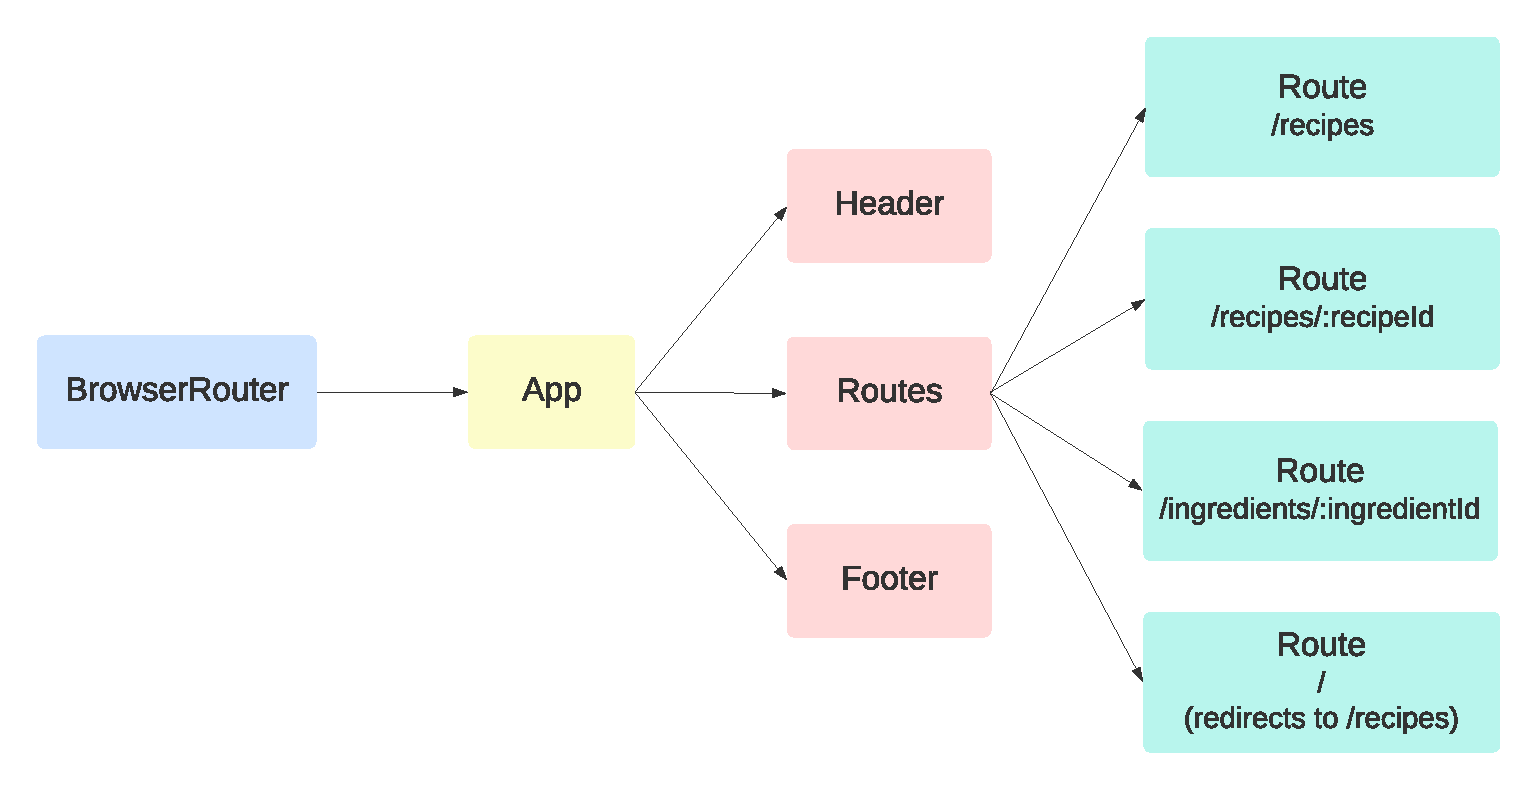
\includegraphics[width=140mm]{../img/react-app}
\caption{Rozhraní aplikace založené na konceptu knihovny React Router.}
\label{obr02:react-app}
\end{figure}

\paragraph{Komponenta vyhledávání receptů}\mbox{}\\

Postup dekompozice si ukážeme na zjednodušeném převodu obrazovky pro vyhledávání receptů na komponenty knihovny React. Obsah celé vyhledávací obrazovky budeme reprezentovat komponentou \texttt{Recipes}. Ta bude zajišťovat mapování filtrů a~současné stránky prohlížení na query parametry URL adresy. Dále bude komunikovat s~REST API, konkrétně s~endpointem pro vyhledávání receptů \texttt{/api/recipes}. Výsledky receptů si vyžádá prostřednictvím asynchronního GET požadavku a~jakmile data obdrží, předá je specializovaným komponentám pro zajištění renderování. Těmito komponentami rozumíme potomky komponenty \texttt{Recipes}.

Jak bylo zmíněno v~začátku této sekce, potomci jsou vnořené komponenty, kterým lze předat data prostřednictvím parametru \texttt{props}. Příkladem vnořené komponenty bude \texttt{RecipesGrid}, která bude dále distribuovat informace o~receptech svým potomkům \texttt{RecipeCard}. Také komponenta \texttt{RecipeCard} bude složena z~menších komponent, konkrétně \texttt{RecipeCardContent}, \texttt{RecipeCardActions} a~\texttt{RecipeCardCollapse}. Rozhraní vyhledávaného receptu bude odpovídat schématu definovanému pro Solr, pojmenujme jej \texttt{SimpleRecipe} pro kontrast s~podrobnějším rozhraním receptu na stránce detailu. Diagram zachycující výše uvedené komponenty včetně parametrů \texttt{props} a~vzájemných vztahů je ilustrován obrázkem \ref{obr02:recipes-component}.

\begin{figure}[h!]\centering
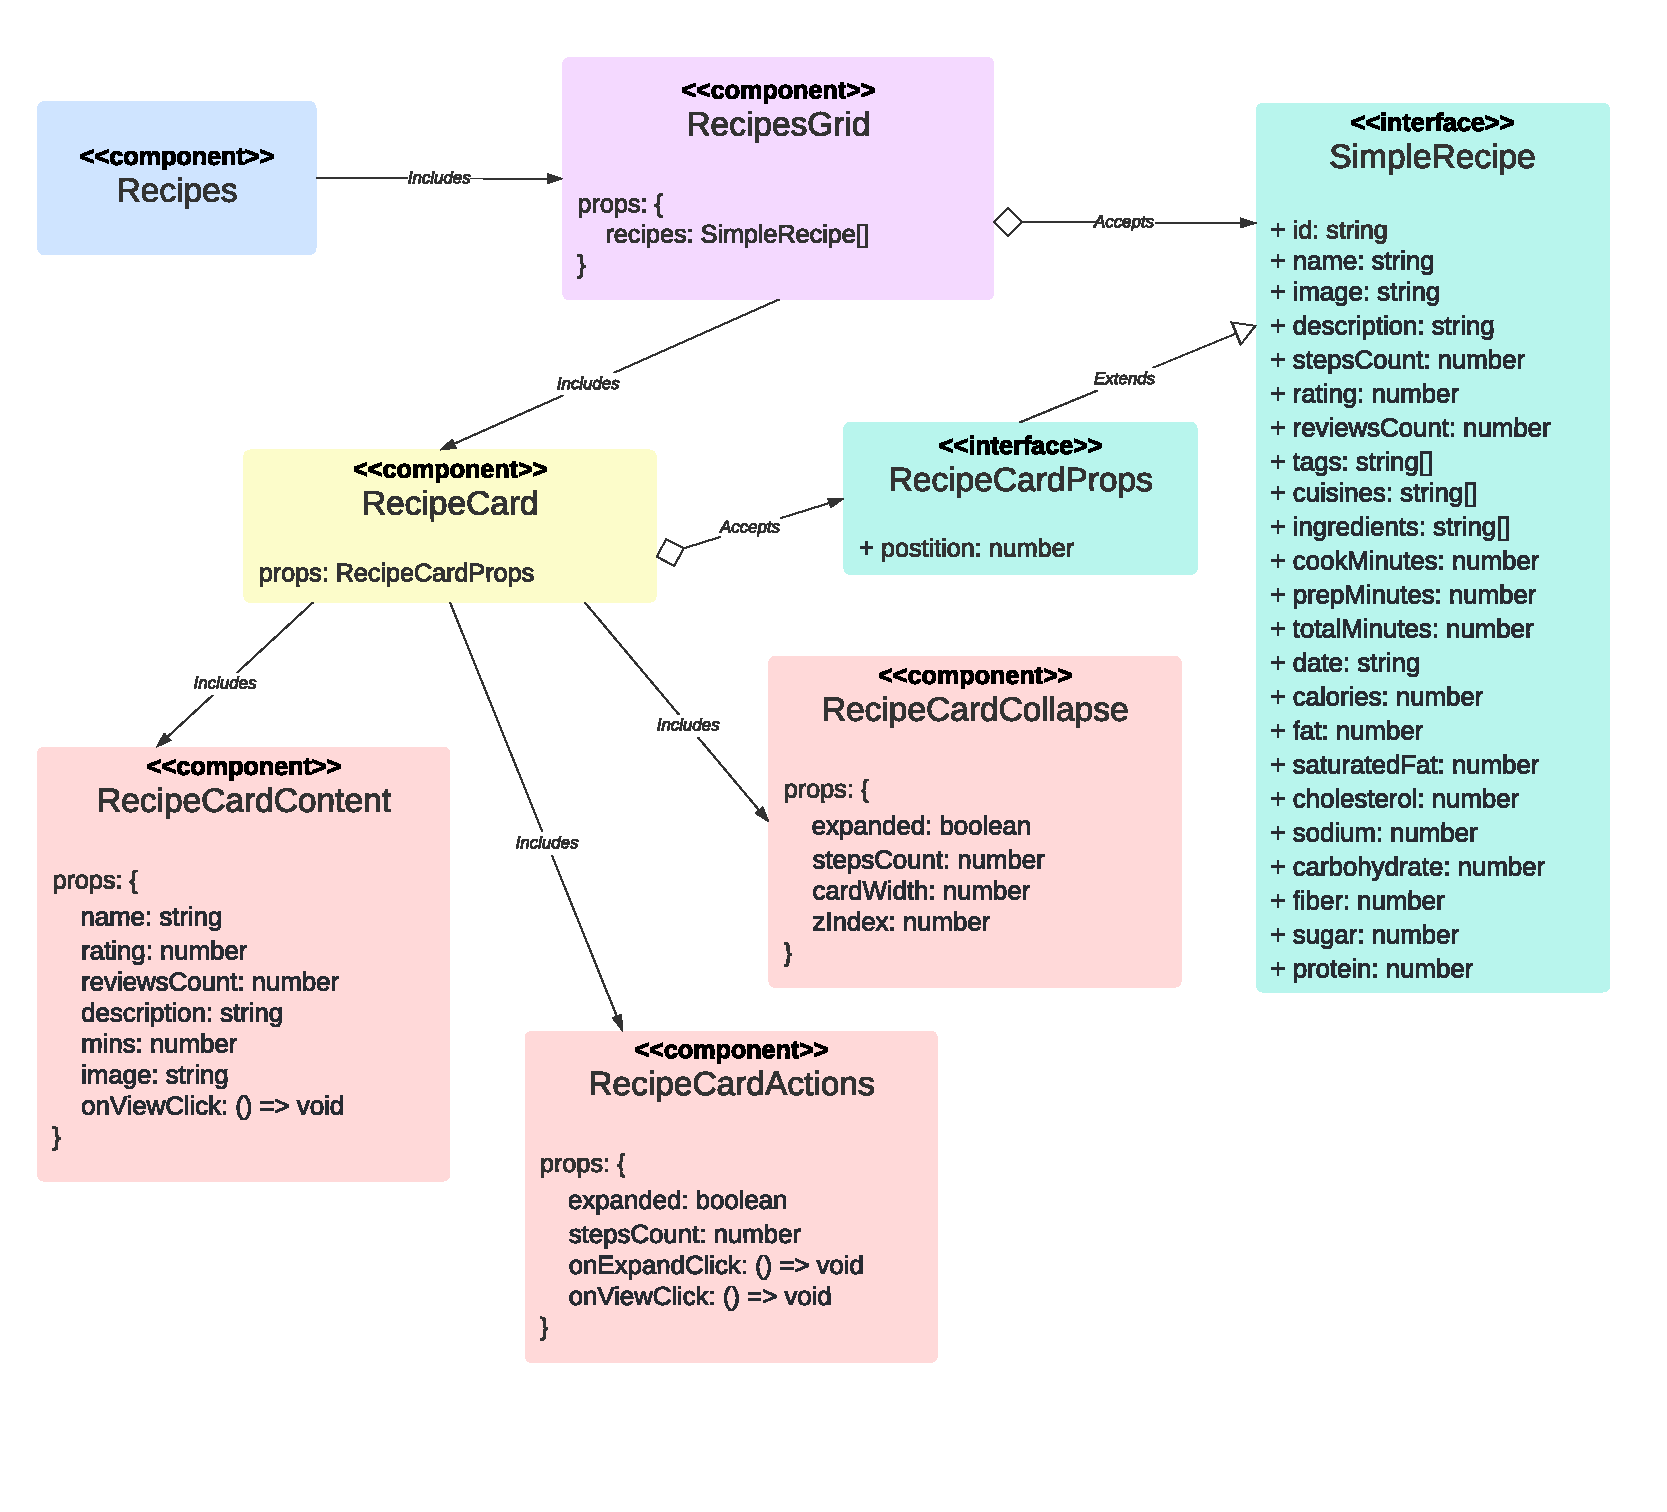
\includegraphics[width=145mm]{../img/recipes-component}
\caption{Diagram znázorňující dekompozici komponenty \texttt{Recipes}.}
\label{obr02:recipes-component}
\end{figure}

Komponenta \texttt{RecipeCardContent} se postará o~zobrazení obrázku, názvu receptu s~úryvkem popisu, hodnocení včetně počtu recenzí a~také času přípravy. Komponenta \texttt{RecipeCardActions} odpovídá spodnímu panelu karty receptu, se kterým lze interagovat. Je zde umístěné tlačítko pro zobrazení receptu a~také tlačítko pro rozbalení seznamu ingrediencí. Samotný seznam ingrediencí již není ve správě komponenty \texttt{RecipeCardActions}. Ta se jen stará o~jeho aktivaci, která je zajištěna zavoláním příslušné funkce předané jako parametr z~rodičovské komponenty \texttt{RecipeCard}. Proměnnou indikující stav rozbalení sekce s~ingrediencemi vlastní komponenta \texttt{RecipeCard}. Při zavolání funkce se tento stav změní a~komponenta \texttt{RecipeCard} předá novou hodnotu komponentě \texttt{RecipeCardCollapse}. Ta na základě aktualizované hodnoty zobrazí nebo skryje seznam ingrediencí.

Finální dekompozice komponenty \texttt{Recipes} bude samozřejmě o~něco složitější, neboť si kromě karet receptů musíme poradit také se zobrazením vyhledávacích filtrů, stránkováním a~nadpisem indikujícím aktuální stav vyhledávání. Rovněž budeme chtít uživatele informovat o~úspěšně přidaných nebo odstraněných filtrech prostřednictvím krátké notifikace. Během implementace uplatníme výše popsané principy dekompozice a~také se pokusíme v~co největší míře zapojit již hotové komponenty poskytované knihovnou Material UI.

\subsection{Alternativní správa dat}

Při návrhu architektury ukládání a~dotazování se nad daty receptů a~ingrediencí bychom se mohli vydat cestou konstrukce vlastního znalostního grafu. Museli bychom definovat ontologii, pomocí které bychom byli schopni kompletně popsat svou doménu receptů i~surovin. Sestrojený graf bychom nahráli do tzv.~\emph{RDF triplestore}, což je typ grafové databáze specializované na jednoduchá RDF tvrzení ve formátu trojic: \emph{subjekt}, \emph{predikát} a~\emph{objekt}. Vrcholy grafu jsou reprezentovány entitami subjektů a~objektů, orientované hrany mezi nimi modelujeme pomocí predikátů. Nad uloženými daty se lze následně dotazovat pomocí jazyka SPARQL, se kterým jsme se setkali při extrakci dat ze znalostních grafů DBpedia a~Wikidata.

\subsubsection{Projekt Linked Recipes}

Výše uvedený přístup byl otestován v~rámci souvisejícího projektu Linked \,Recipes\footnote{https://github.com/lhotanok/LinkedRecipes}, který vznikl jako semestrální práce v~předmětu Data na Webu vedeném RNDr.~Jakubem~Klímkem,~Ph.D. v~roce $2022$. Součástí projektu bylo získání dat s~recepty ze $3$~různých zdrojů, dále jejich převedení do RDF formátu v~libovolné serializaci, nalezení linků mezi datasety navzájem i~s~externími grafy a~na závěr vytvoření jednoduché aplikace, která všechna data propojila a~umožnila nad nimi spouštět SPARQL dotazy. Jako statické zdroje dat byly vybrány datasety Food.com Recipes and~Interactions a~BBC Recipes. Ty byly obohaceny o~dataset vygenerovaný z~webové aplikace Allrecipes a~jako zástupci externích grafů byly zvoleny projekty DBpedia a~Wikidata. Je zde tedy velký překryv s~datovými sadami využívanými v~naší aplikaci pro vyhledávání receptů.

Aplikace Linked Recipes je napsána v~jazyce Java a~pro obsluhu HTTP požadavků využívá koncept tzv.~servletů, které generují odpovídající HTML dokumenty, často na základě komunikace s~databází. Aplikace používá RDF triplestore jako úložiště dat, konkrétně implementaci frameworku Eclipse RDF4J. Data ve formátu RDF jsou při spuštění aplikace nahrána do paměti prostřednictvím úložiště \emph{MemoryStore}, které je dle dokumentace třídy vhodné pro dataset s~méně než $100\,000$ tvrzeními. Alternativně lze použít úložiště provázané se SPARQL endpointem, který přijímá dotazy přes HTTP.

Aplikace si díky RDF triplestore a~SPARQL dotazům dokáže poměrně snadno poradit s~vyhledáním receptů dle ingrediencí, včetně zákazu vybraných ingrediencí. Také zvládá filtrovat recepty na základě povoleného rozmezí nutričních hodnot. Dalším v~aplikaci demonstrovaným příkazem je sestavení grafu ingrediencí s~využitím dat z~grafu Wikidata. Aplikace má k~dispozici seznam entit z~Wikidata, které se namapovaly na ingredience datasetů s~recepty. Přímo za běhu pak získává odkazy na obrázky k~daným ingrediencím a~vkládá je do HTML dokumentu. Nepotřebuje si tedy data k~ingrediencím z~Wikidata ukládat do interní databáze, čímž se zjednoduší architektura aplikace. Nevýhodou je ale podstatně delší čas potřebný k~získání a~zobrazení informací.

Pokud bychom se rozhodli pro stejný návrh aplikace jako v~projektu Linked Recipes, nahradili bychom vrstvy CouchDB a~Solr úložištěm RDF triplestore. To by v~sobě mělo uložena všechna data stejně jako CouchDB a~zároveň by řešilo vyhledávací dotazy namísto platformy Solr. Rychlost vyhledávání by byla závislá pouze na optimalizaci SPARQL dotazů. Narazili bychom na problém, pokud bychom se nespokojili s~vyhledáváním dle přesné shody a~vyžadovali chytřejší řešení po vzoru Solr a~jeho vyhledávání v~anglickém textu. Dále bychom se museli vypořádat s~požadavkem fasetového vyhledávání, pro které máme v~Solr přímou podporu na straně serveru. Fasetové vyhledávání se obvykle nepoužívá v~přímé kombinaci s~RDF modelem z~důvodu rizika, že by příkazy potřebné k~jeho podpoře byly příliš komplexní a~jejich výkon nedostačující \citep{sparql-facet}. Sehnat dostatečně výkonné a~dobře zdokumentované řešení by tedy bylo podstatně složitější v porovnání s~využitím osvědčeného Solr nebo jeho alternativ v~podobě ElasticSearch\footnote{https://www.elastic.co/guide/en/app-search/current/facets-guide.html} či Sphinx\footnote{http://sphinxsearch.com/blog/2013/06/21/faceted-search-with-sphinx/}.